% Williams Physics Thesis template
% Patterned after the work of Cole Meisenhelder '15
% Commented by Prof. Charlie Doret, 12/2016

\documentclass[12pt, oneside]{book} 

% The \usepackage{} command will import predefined fonts, symbols, environments, etc.  For example, the ams packages below come from the American Mathematical Society and include all kinds of useful math symbols like integrals
\usepackage{amscd}
\usepackage{amsmath}
\usepackage{amssymb}
\usepackage{amsthm}
\usepackage{verbatim}
\usepackage[utf8]{inputenc}
\usepackage{geometry}                		% See geometry.pdf to learn the layout options. There are lots.
\geometry{letterpaper}                   		% ... or a4paper or a5paper or ... 
%\geometry{landscape}                		% Activate for for rotated page geometry
\usepackage[pdftex]{graphicx}				% Use pdf, png, jpg, or eps� with pdflatex; use eps in DVI mode	
\usepackage{setspace}
\usepackage{physics}
\usepackage{subcaption}
\usepackage[numbers]{natbib}
\usepackage{pdfpages}
\usepackage{bm}

\usepackage{wrapfig}				% enables the use of \wrapfig, for figures with text wrapped around them
%\usepackage{lipsum}			% gives access to \lipsum, which dumps some latin text into your document as filler if you want to check formatting

%\usepackage[parfill]{parskip}    		% Activate to begin paragraphs with an empty line rather than an indent

\usepackage{hyperref}
\hypersetup{
	colorlinks=true, %set true if you want colored links
	linktoc=all,     %set to all if you want both sections and subsections linked
	allcolors = black %get rid of weird auto link highlighting
}
% \usepackage{sidecap}
% \usepackage[colorinlistoftodos]{todonotes}
\usepackage{fancyvrb} %useful for codeblocks not being split
\usepackage{multicol}
% \usepackage[hashEnumerators,smartEllipses]{markdown}

\usepackage{pmboxdraw}  %needed for code file tree symbols
% for code blocks -------
% \usepackage{listings}
% \usepackage{color}
% \definecolor{dkgreen}{rgb}{0,0.6,0}
% \definecolor{gray}{rgb}{0.5,0.5,0.5}
% \definecolor{mauve}{rgb}{0.58,0,0.82}
% \lstset{frame=tb,
%   language=Python,
%   aboveskip=3mm,
%   belowskip=3mm,
%   showstringspaces=false,
%   columns=flexible,
%   basicstyle={\small\ttfamily},
%   numbers=none,
%   numberstyle=\tiny\color{gray},
%   keywordstyle=\color{blue},
%   commentstyle=\color{dkgreen},
%   stringstyle=\color{mauve},
%   breaklines=true,
%   breakatwhitespace=true,
%   tabsize=3
% }
% -------

\newcommand*{\boxednumber}[1]{%
    \expandafter\readdigit\the\numexpr#1\relax\relax
}
\newcommand*{\readdigit}[1]{%
    \ifx\relax#1\else
        \boxeddigit{#1}%
        \expandafter\readdigit
    \fi
}
% Format macro used for every digit, adjust to your liking:
\newcommand*{\boxeddigit}[1]{\fbox{#1}\hspace{-\fboxrule}}

% Here we set the page dimensions to match the standard thesis format.  These values should not be changed.
%%% SET LENTGH AND WIDTH %%%
\setlength{\textwidth}{6.5in}
\setlength{\textheight}{8.5in}
\setlength{\oddsidemargin}{0pt}
\setlength{\evensidemargin}{0pt}
\setlength{\topmargin}{0pt}
\setlength{\marginparsep}{0pt}
\setlength{\marginparwidth}{1in}

%\begin{document} starts LaTeX looking for actual content.  Everything above this point is purely formatting.
\begin{document}

\begin{titlepage}
\begin{center}

% \vspace* creates some vertical white space on the page to make the title page look more pleasing.  \vspace would do much the same thing, but would not insert the white space if we were at the top of a fresh page.  As this is the start of the document we're obviously at the beginning of a page, so the asterisk is necessary to ensure we still put in two cm of white space.
\vspace*{2cm}

{\huge Investigation of Bond Strain Effects\\on XANES Spectra by \\Supervised Machine Learning} % \huge sets the font size.  Other options include things like \large, \Large, \small, \tiny, etc.

\vspace{2cm}

{\large by\\Jeremy K. Thaller}

\vspace{2cm}

%% Centered version
% \begin{multicols}{2}
% 	Professor Anatoly Frenkel, Advisor \hfill \\
% 	Brookhaven National Laboratory \hfill \\
% 	Chemistry Division \hfill \\
% 	\columnbreak
% 	Professor Wolfgang Schmahl, Advisor \\
% 	Ludwig-Maximilians-Universität München \\
% 	Fakultät Geowissenschaft
% \end{multicols}

\noindent\begin{tabular}[t]{@{}l}
	Professor Anatoly Frenkel, Advisor\\
	Brookhaven National Laboratory\\
	Chemistry Division \\
	New York, USA
\end{tabular}
\hfill
\begin{tabular}[t]{l@{}}
% \begin{tabular}[t]{r@{}}
	Professor Wolfgang Schmahl, Advisor \\
	Ludwig-Maximilians-Universität\\
	Fakultät Geowissenschaft \\
	München, Germany
\end{tabular}

% \vfill creates an arbitrary amount of vertical white space as necessary to fill the page
\vfill

A Master thesis submitted to the Faculty
of Earth- and Environmental Sciences\\
of Ludwig-Maximilians-Universität München
in the framework of MaMaSELF

\vspace*{3cm}

% Brookhaven National Labs\\
% Brookhaven, New York\\
\today % you might choose to set a permanent date, but \today will put in today's date
\end{center}
\end{titlepage}

% \frontmatter defines the pieces of the thesis which will use roman numerals for page numbering
\frontmatter 


% \chapter{} and/or \chapter*{} will create a chapter in your thesis.  Including the asterisk will cause the chapter to not appear in the table of contents.

% \input will reference a particular .tex file.  Here we are grabbing a file entitled Abstract stored in the folder Chapters
\chapter{Abstract}
% Here is where you'll include the actual text for your abstract.  Because this lives inside the main document and will be included with a \input command, no tags are needed to start a new document.  Instead, just type.


% Your abstract will summarize your thesis in one or two paragraphs.  This brief summary should emphasize methods and results, not introductory material.

% X-ray absorption spectroscopy (XAS) is a widely used experimental technique for material characterization. The two
A recently published method \cite{Timoshenko2017} enables the decoding of X-ray absorption near edge structure (XANES) spectra of nanoparticles to obtain important structural descriptors: coordination numbers and bond distances. Utilizing supervised machine learning (ML), the method trains an artificial neural network (ANN) to recognize a relationship between the nanoparticle structure and the XANES spectrum. Once trained, the ANN is used to ``invert'' an unknown spectrum to obtain the corresponding descriptors of the catalyst structure. Bond strain is known to be an important catalytic descriptor, yet, its accurate determination in reaction conditions is hampered by high temperature and low weight loading of real catalysts. ML–assisted XANES analysis offers a promising new direction for extracting the bond strain information from XANES---and not from extended x-ray absorption fine structure (EXAFS) analysis. Using simulated XANES spectra of Au nanoparticles, we have developed an ANN capable of ``inverting'' an unseen XANES spectrum and predicting structural disorder in the form of mean-squared displacement. The utility of the method was demonstrated on both the computer-simulated nanoparticles of different sizes and degrees of disorder, as well as on experimental data of disordered nanoparticles.

% Further, the network is being trained to predict additional disorder descriptors, which would allow for the reconstruction of the radial distribution function, $g(r)$. This prediction is possible in part due to a new statistical averaging approach whereby XANES spectra of disordered structures are created from simulated XANES spectra of non-disordered structures.

% https://www.worldscientific.com/doi/abs/10.1142/9789811204579_0007
% Y. Lin, M. Topsakal, J. Timoshenko, D. Lu, S. Yoo, A. I. Frenkel
% Machine-Learning assisted structure determination of metallic nanoparticles: A benchmark
% In: Handbook on Big Data and Machine Learning in the Physical Sciences, World Scientific Series on Emerging Technologies, v.2, Chapter 7, pp. 127-140 (2020).
\chapter{Executive Summary}
% Here we have your executive summary.

% Your executive summary will give a detailed summary of your thesis, hitting the high points and perhaps including a figure or two.  This should have all of the important take-home messages; though details will of course be left for the thesis itself, here you should give enough detail for a reader to have a good idea of the content of the full document.  Importantly, this summary should be able to stand alone, separate from the rest of the document, so although you will be emphasizing the key results of your work, you will probably also want to include a sentence or two of introduction and context for the work you have done.

This thesis presents work toward developing an artificial neural network (ANN) capable of ingesting a XANES spectrum and predicting the mean squared displacement (MSD) of the structure. A schematic of this network is presented in Figure \ref{fig:thesis-design}. 

\begin{figure}[h!]
    \centering
    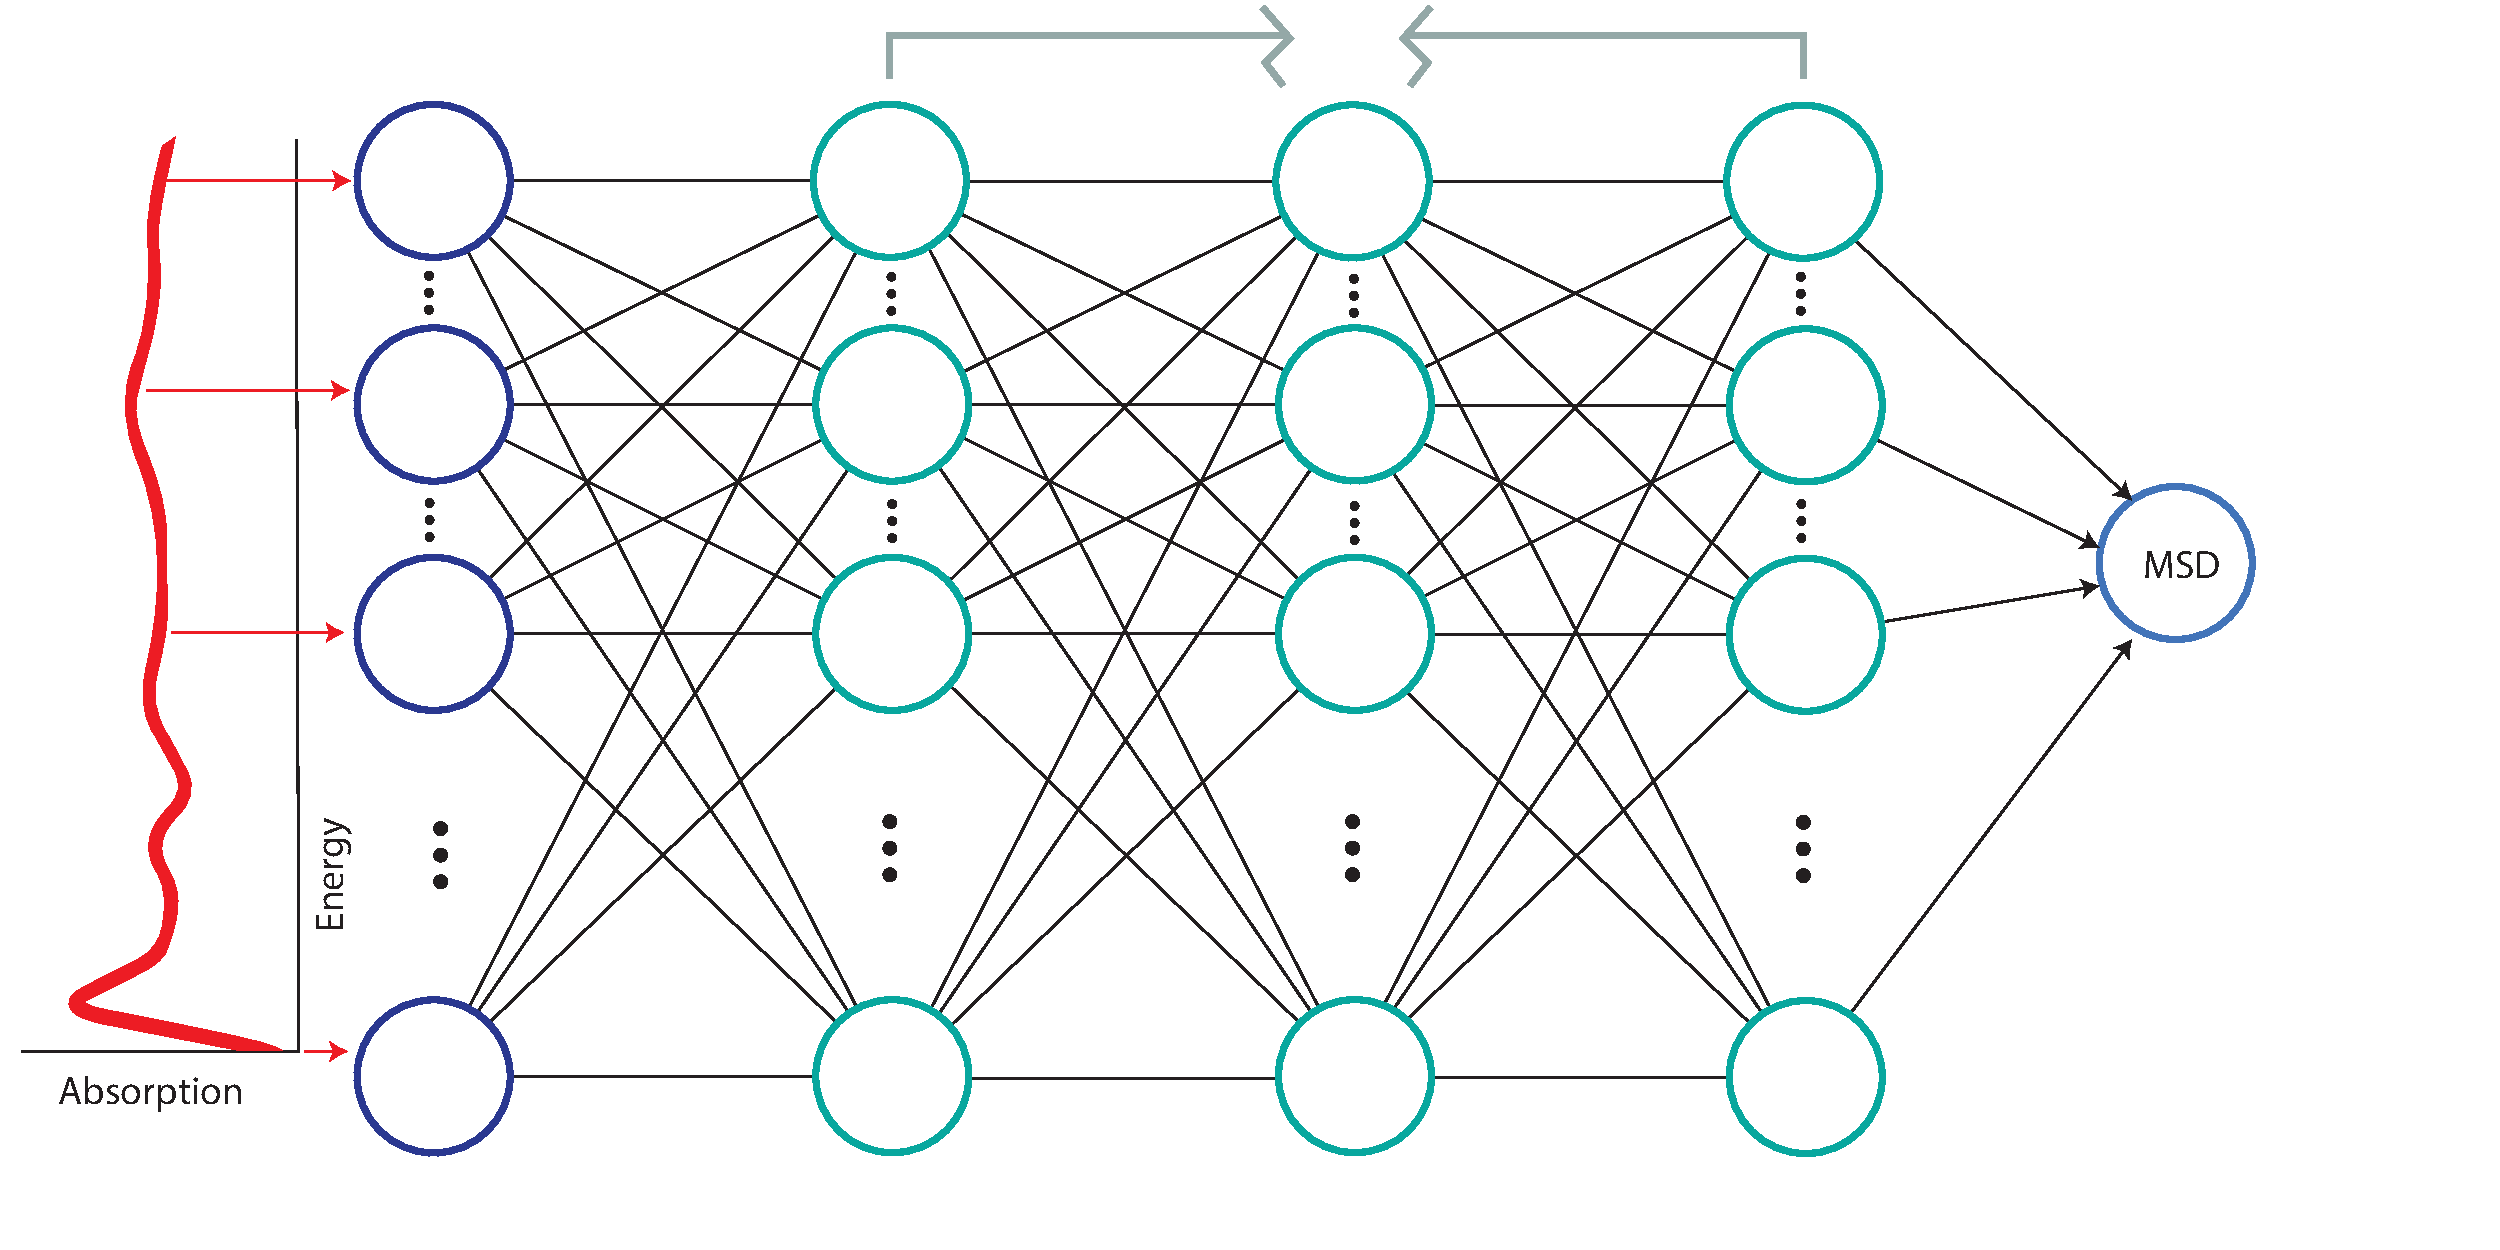
\includegraphics[width=\linewidth]{Chapters/Figures/thesis-design.pdf}
    \caption[Project Approach]{The above figure describes the general structure of the neural network described in this thesis. The model inputs the absorption values for a XANES spectrum and predicts the mean squared displacement (MSD) of the structure. For this thesis, we train the network exclusively on large, bulk-like gold nanoparticles.}
    \label{fig:thesis-design}
\end{figure}

In order to train a neural network, we rely on a large quantity of data obtained through FEFF9 \cite{feff-citation}, an $ ab~initio $ x-ray absorption simulation software capable of simulating XANES spectra. We first present work on developing a new, statistical-based methodology for simulating disordered structures. The goal of this new approach was to reduce the number of required simulations for creating a dataset of FEFF-simulated structures. Instead of simulating the disorder structures themselves, different isotropically ``expanded'' or ``contracted'' configurations were created and simulated. A tunable, distributed weighted average of these resulted was then used to approximate the absorption spectrum of disordered structures. This method, however, was ultimately abandoned for the remainder of this thesis due to systematic discrepancies between its results and those of the traditional simulation approach. 

Trained on the simulation data, the neural network shows great predictive accuracy and promise for predicting the mean squared displacement and mean location of nearest neighbor bond lengths in Au, bulk-like nanoparticles. In order for the neural network to make predictions from experimental data---as opposed to simulation data---we employ a technique in machine learning known as ``one-shot transfer learning.'' The process is the topic of current work, and we end the thesis with a discussion on the transfer-leaning plan and progress made towards this goal.


\begin{figure}
    \centering
    \includegraphics[width=\linewidth]{Chapters/Figures/nn_rdf_validation_preds-fixed-just-msd-and-mean.png}
    \caption[Simulation Test Set Predictions]{The predictions for a train-test split on particle-averaged simulation data are presented above. Each point in each subplot represents a FEFF simulated spectrum in the test set. For each spectrum, the y-axis represents the MSD value predicted by the NN, and the x-axis represents the true label (MSD for the left figure and mean for the right) for that spectrum. Hence, points on the $ y=x $ red line are perfect predictions.}
    \label{fig:train-test-split-just-msd-and-mean}
\end{figure}


\chapter{Acknowledgments}
% Here we have a section where you might choose to acknoweldge your family, fellow students, advisor, dog, etc.

I would like to thank my advisor Professor Anatoly Frenkel and my professors in Germany and Poland over the past two years. I also owe a great debt of gratitude towards those who took the time to help proofread my work, as well as the free and open-source software (FOSS) community.

%\tableofcontents will create a table of contents.  By default it will include entries for any \chapter, \section, and \subsection command that appears in your thesis unless you have called the tag with an asterisk
\tableofcontents

\listoffigures

% \mainmatter defines the main body of the thesis and marks where regular numbering will begin
\mainmatter

\chapter{Introduction}
% Look!  A mock introduction

The introduction is one of the most important pieces of your thesis.  Here is a place for you to introduce the problem(s) on which you have worked and place them in the larger context of your field.  You should aim to ensure that this section is completely understandable to virtually anyone - and certainly anyone with a sophomore-level grasp of physics.  Presumably this will include references to the literature.

In addition to setting your work into context, a second good idea for your introduction is to give a short outline for what the rest of your thesis will discuss.  This is often done in the closing paragraph(s) of the introduction with sentences like ``In the following chapters \ldots " and ``Chapter 2 discusses \ldots"  Tremendous detail is not required in this outline, but rather just a brief road map for the rest of the document.

\section{Traditional XANES}

The \texttt{\textbackslash section} tag will create a new section within a chapter.  Sections will be sequenced with digits following a decimal point in the table of contents, i.e. this is section 1.1.


\section{Machine Learning in Science}


Probably want to talk about these papers in this section \cite{timoshenko2018neural} \cite{Timoshenko2017}.



% \chapter{XAFS In Depth}
\chapter{Simulating Disorder}
% Another mock chapter

Here is a second mock chapter.  As far as the \LaTeX ~is concerned, it is in no way different from the introduction excepting that it appears after it in the main .tex file.  As before, it can be populated with sections, subsections, figures, etc. as you see fit.

In fact, you will probably write perhaps three to six chapters for your thesis depending on how your work is most effectively organized.  Most theses will contain an introduction, at least one `body' chapter, and some sort of conclusions/future directions chapter.  Most theses will also include an appendix or two \ldots

\section{Autoencoders}
Talk about how autoencoders work. Give a nice broad explanation and really go into the math. Include some nice diagrams

Here's \cite{ng2011sparse} a good source to read and model off of. Here \cite{Bhowick2019} is another paper that might be interesting to read. It's about getting noise free data from the original data using an autoencoder. Neat idea, and could actually be very relevant because they're using geophysical data.

\chapter{Machine Learning}
%Chapter 3
I think results and discussion of results should go here

\chapter{Results}
% Results
The results of the training process are presented in this chapter. We begin by first outlining the training network architecture and training process on simulated XANES in section \ref{sec:nn-sim-data}. Then, we discuss the work on expanding the model to make solid predictions on experimental data.

\section{Training with Simulation Data} \label{sec:nn-sim-data}

The 1000 simulated XANES spectra were first loaded into a Pandas dataframe \cite{pandas-1} \cite{pandas-2} of shape $ 1000\times82 $. Each of the 82 columns represents a discrete energy value, and each row represents the absorption for a given spectrum at those energies. The dataset was split into training and testing groups according to an 80-20 random split, respectively. All absorption columns were then scaled via the standard scalar (\ref{z-score}) and the training labels scaled via a min-max scaler (\ref{eqn:min-max-scaler}). First, the model was trained to predict four descriptors: the mean squared displacement (MSD), the mean bond length distance, the standard deviation of the bond length distributions, and the skew of the bond length distribution. Note that the standard deviation is equal to the square root of the MSD. This feature was only included preliminarily in order to better understand the correlation in the network's predictions. 

\bgroup
\def\arraystretch{1.5}%  1 is the default, change whatever you need
\begin{table}[h!]
    \centering
    \begin{tabular}{|l|l|l|}
    \hline
    \textbf{Layer  Type }   & \textbf{ Output Shape}  & \textbf{\# of Parameters} \\ \hline
    Normalization  & (None, 82)    & 165                  \\ \hline
    Dense          & (None, 128)   & 10,624               \\ \hline
    Dense          & (None, 128)   & 16,512               \\ \hline
    Dense          & (None, 512)   & 25,088               \\ \hline
    Reshape        & (None, 8, 64) & 0                    \\ \hline
    1D-Convolution & (None, 6, 32) & 6,176                \\ \hline
    Dropout        & (None, 6, 32) & 0                    \\ \hline
    1D-Max-Pooling & (None, 3, 32) & 0                    \\ \hline
    Flatten        & (None, 96)    & 0                    \\ \hline
    Dense          & (None, 128)   & 12,416               \\ \hline
    Dense          & (None, 48)    & 6,192                \\ \hline
    Dense          & (None, 512)   & 25,088               \\ \hline
    Flatten        & (None, 512)   & 0                    \\ \hline
    Dense          & (None, 4)     & 513                  \\ \hline
    \end{tabular}
    \caption[NN-Architecture Optimized for Simulations]{The model architecture for the network trained entirely on simulation data (which performed poorly on experimental data) relies primarily on affine (Dense) and convolutional layers. The model includes 108,966 total parameters, 108,801 of which are trainable.}
    \label{tb:nn-arch-sims}
\end{table}
\egroup


\begin{figure}
    \centering
    \includegraphics[width=\linewidth]{Chapters/Figures/pa_train-test-fixed.png}
    \caption[Simulation Test Set Predictions]{One configuration of the trained neural network includes four output nodes: MSD, Sigma, Mean, and Kurtosis. Sigma is the square root of the MSD and was included during training to confirm the patterns recognized by the network. Each point in each subplot represents a FEFF simulated spectrum in the test set. For each spectrum, the y-axis represents the MSD value predicted by the NN, and the x-axis represents the true MSD (label) for that spectrum. Hence, points on the $ y=x $ red line are perfect predictions.}
    \label{fig:train-test-split-all4}
\end{figure}

\section{Experimental Data} \label{ch:results}

Training a neural network entirely on simulation data and then making predictions on experimental data is unlikely to provide quality results. Using the trained network from Table (\ref{tb:nn-arch-sims}) that predicted the test set values in Figure \ref{fig:train-test-split-all4}, we predicted the MSD values from two experimental spectra. On the unpublished IMASC data, the network predicted an MSD of $0.0003724~\text{\AA}^2$ instead of the EXAFS equation fitted value of ${\sigma^2=0.0102(8)~\text{\AA}^2}$. This poor prediction suggests the network considers the experimental spectrum to look most similar to the lowest disorder FEFF spectra; the model is not generalizing to understand the disorder encoded in the spectral shape.


\begin{figure}
    \centering
    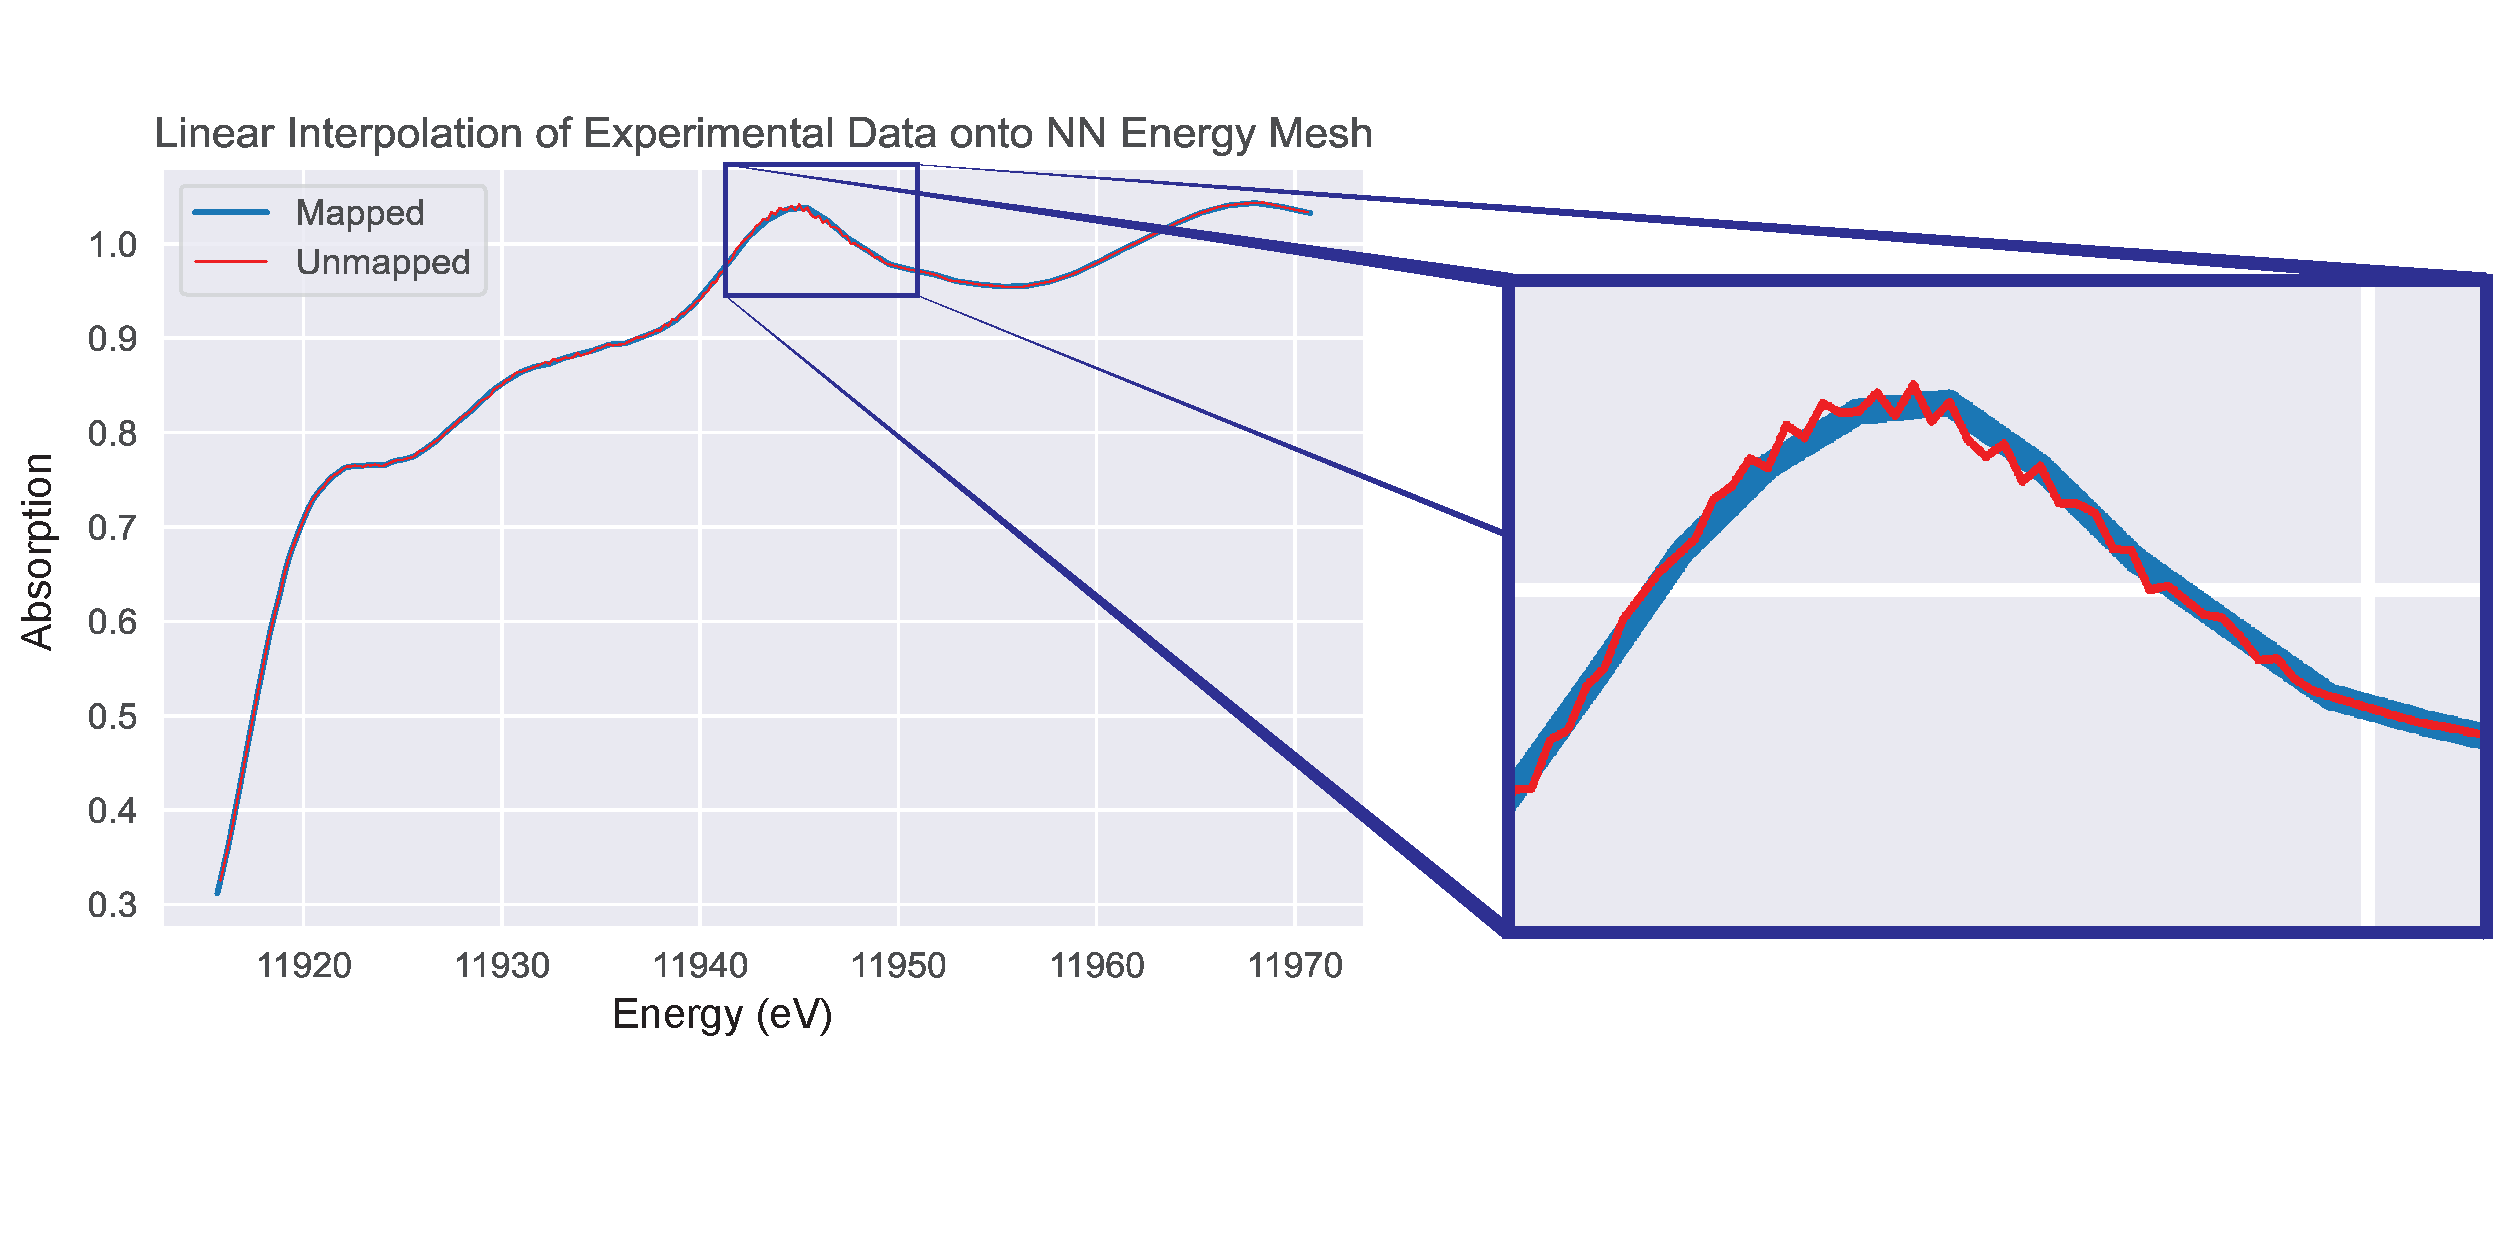
\includegraphics[width=\linewidth]{Chapters/Figures/quality-of-interpolation-skinny.pdf}
    \caption[Experimental Data Interpolation]{The experimental data is measured as a function of different energy values than those on which the neural network is trained. Consequently, the experimental spectrum must be mapped onto the proper energy mesh via linear interpolation.}
    \label{fig:interpolation-skinny}
\end{figure}

\subsection{Data Augmentation}
While there is ample data for training and predicting on only simulation data, we only have two experimental spectra. In order to create more training and testing data for the neural network, two types of data augmentation were utilized: Gaussian noise inclusion and horizontal spectral shifting. While the motivation for utilizing data augmentation is to expand the size of the experimental training and testing set, the neural network must be trained to recognize the augmentation types prior to training or testing on the experimental data. As such, both the FEFF simulated dataset and experimental dataset are augmented.

Noise is artificially injected into the spectra by randomly shifting each absorption coefficient vertically. The shifted value for each energy level is selected from a Gaussian distribution with standard deviation $ \sigma=0.01 $. An exaggerated example of the injected noise is shown in Figure \ref{fig:data-aug-gauss-noise}.

\begin{figure}[h!]
    \centering
    \includegraphics[width=.75\linewidth]{Chapters/Figures/gaussian-noise-data-aug.pdf}
    \caption[Data Augmentation: Gaussian Noise]{Gaussian noise is added to the spectra to increase the variance of the training data. This helps the network to learn the low-level features of the spectra and ignore artifacts not caused by the structural disorder. For demonstration purposes, the scale of the noise in this figure has been increased beyond what was used in training.}
    \label{fig:data-aug-gauss-noise}
\end{figure}

The second form of data augmentation utilizes horizontal shifts. While this is common for signal processing and time series analysis, the inclusion here is more controversial. In XAFS, the edge location is dependent on the oxidation/reduction state of the species. Shifting the horizontal location is akin to shifting the species of the model; however, the neural network is not being tasked to determine the oxidation state of the sample. Instead, the model is merely tasked with predicting the mean squared displacement of the nanoparticle's bond lengths. The theory is that the disorder information is encoded throughout the entire XANES spectrum, not from just a simple feature such as the edge placement.  

\begin{figure}[h!]
    \centering
    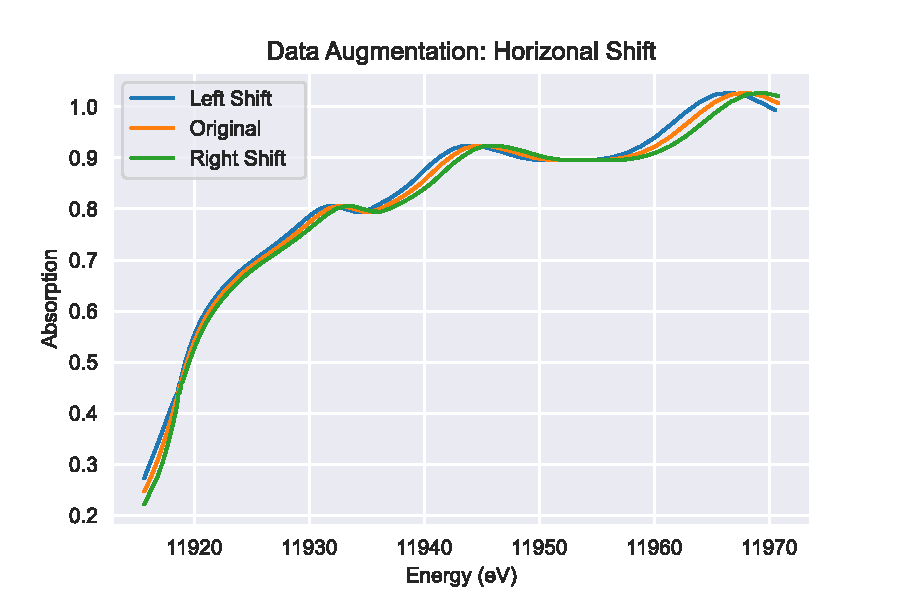
\includegraphics[width=.75\linewidth]{Chapters/Figures/horz-shift-3way.pdf}
    \caption[Data Augmentation: Horizontal Shift]{In order to train the network to predict disorder from the overall shape of the spectra---as opposed to fixating on the edge location---we introduce horizontal-shift as a data augmentation technique.}
    \label{fig:data-aug-hor}
\end{figure}

\subsection{Transfer Learning}
In building the transfer learning model, we opted to begin with a new network architecture, which can be found in Table (\ref{tab:meta-1}). We hypothesized that applying convolutional layers before any affine layers may lead to a more consistent prediction between simulation and experimental spectra.

\begin{figure}
    \centering
    \includegraphics[width=\linewidth]{Chapters/Figures/transfer-learning-breakdown.pdf}
    \caption[Transfer Learning Process]{The allocation of training and testing data is summarized above. At each stage, the network architecture remains unchanged; however, some of the network's parameters are retrained on new data. The different sets of data are color-coded for readability. Note that the network is never trained on the original experimental data---it is only used for the final stage of testing.}
    \label{fig:transfer-learning-databreakdown}
\end{figure}

\bgroup
\def\arraystretch{1.5}
\begin{table}[]
    \centering
        \begin{tabular}{|l|l|l|l|}
        \hline
        \multicolumn{1}{|c|}{\textbf{Name}} & \multicolumn{1}{c|}{\textbf{Type}} & \multicolumn{1}{c|}{\textbf{\# Parameters}} & \multicolumn{1}{c|}{\textbf{Output Shape}} \\ \hline
        normalization\_input                & InputLayer                         & 0                                           &                                            \\ \hline
        normalization                       & Normalization                      & 165                                         & None, 82                                   \\ \hline
        reshape                             & Reshape                            & 0                                           & None, 82, 1                                \\ \hline
        conv1                               & Conv1D                             & 128                                         & None, 82, 32                               \\ \hline
        max\_pooling1d                      & MaxPooling1D                       & 0                                           & None, 41, 32                               \\ \hline
        conv2                               & Conv1D                             & 3104                                        & None, 39, 32                               \\ \hline
        max\_pooling1d\_1                   & MaxPooling1D                       & 0                                           & None, 19, 32                               \\ \hline
        flatten                             & Flatten                            & 0                                           & None, 608                                  \\ \hline
        dense1                               & Dense                              & 58464                                       & None, 96                                   \\ \hline
        dout                                & DropOut                            & 0                                           & None, 96                                   \\ \hline
        dense2                              & Dense                              & 30264                                       & None, 312                                  \\ \hline
        output                              & Dense                              & 313                                         & None, 1                                    \\ \hline
    \end{tabular}
    \caption{A new network architecture was constructed for the transfer learning process. The new network only has one output node, representing the MSD of the input spectrum.}
    \label{tab:meta-1}
\end{table}
\egroup


Our approach for applying transfer learning involves two stages of fine-tuning. First, we primarily train the model on FEFF simulated spectra, selecting an architecture and hyperparameters which are likely to be compatible with fine-tuning. We achieve this by weighting the validation set heavily (around $ 10\% $) with augmented experimental spectra and choosing a model which predicts unseen data-augmented experimental spectra as well as it predicts unseen simulated FEFF spectra. The training loss curves and selection process can be found in Figure \ref{fig:meta-1-sweep-loss}. One concern with this approach is that we are injecting biases into our model selection; however, we take this into account through the utilization of a third, unseen test set and the fact that the model does not update its parameters based on its validation set predictions. When training a model in machine learning, the parameters are continuously updated until a minimum is reached in the loss function. While the loss landscape will have a global minimum, it also contains local minima, some of which will be more agnostic to the differences in experimental spectra and be better candidates for transfer learning. In this first stage of learning, the intention is to teach the model to find broad predictive features from the simulation set while selecting a model at a local minimum that is likely to be a successful transfer-learning candidate. 


\begin{figure}
    \centering
    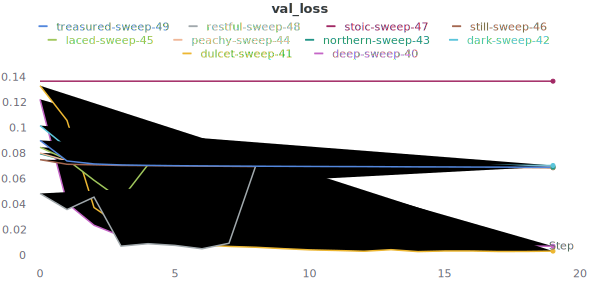
\includegraphics[width=\linewidth]{Chapters/Figures/10-sweep.png}
    \caption[Hyperparamater Sweep: Cost Curve]{The validation cost (mean-squared-error) for 10 out of the 50 hyperparameter combinations searched in this sweep are plotted above. Most hyperparameters result in a loss curve stabilizing around 0.08, which is significantly higher than the training cost (not shown) that stabilized around 0.01. A few of the validation loss curves, instead, stabilized around 0.01 (dulcet-sweep-41 and deep-sweep-40). Because the validation set is heavily weighted with augmented experimental spectra, these two spectra are likely to be good candidates for transfer learning onto experimental data.}
    \label{fig:meta-1-sweep-loss}
\end{figure}

The next stage of transfer learning seeks to teach the model to ignore noise and focus on the broader shape of the spectrum. We achieve this by freezing the early stages of the model and retraining the later parameters on a new dataset comprised primarily entirely of data-augmented spectra. Often, models are trained with the augmented dataset in the initial stage, which helps act as a form of regularization. In the case of transfer learning, however, applying this regularization so early on in the process may lead to undesirable local minima for which transfer learning onto the experimental dataset would be impossible. By applying an initial stage of fine-tuning to a well-tuned base model, we increase the likelihood of a successful second fine-tuning stage.

The last stage of the fine-tuning process is to freeze even more layers and reduce the learning rate, then train the model using all of the data-augmented experimental spectra. If the process is successful, the model will have learned to predict the MSD and ignore horizontal and Gaussian noise in the spectra from the first stage. In this way, we have increased the number of possible training samples to use for the final fine-tuning stage from one to many, allowing us to withhold both of the un-altered experimental spectra from the training process and use them to evaluate the success of the transfer learning process. A visualization and specific breakdown of which data is allocated into each stage of the training process can be found in Figure \ref{fig:transfer-learning-databreakdown}.

\begin{figure}
    \centering
    \includegraphics[width=\linewidth]{Chapters/Figures/new-hyperparameter-sweep-meta-1.png}
    \caption[Hyperpamater Sweep: Graphical Representation]{The hyperparameters are obtained through a ``sweep,'' where the entire training process (20 epochs) is repeated with different hyperparameters each time. The hyperparameter training process and figure generation was conducted with the aid of \cite{wandb}.}
    \label{fig:meta-1-sweep-params}
\end{figure}


\begin{figure}
    \centering
    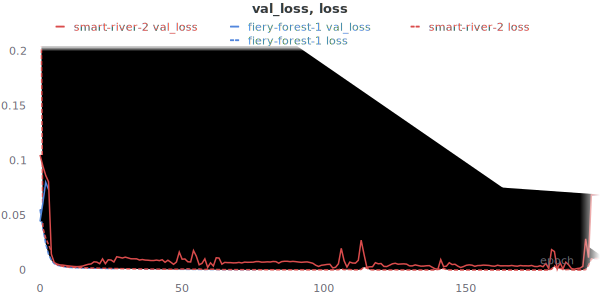
\includegraphics[width=\linewidth]{Chapters/Figures/best-params-meta1.png}
    \label{fig:meta-1-best}
    \caption[Learning Curve for the best hyperparameters]{Both iterations of the training process were run with identical network architectures and hyperparameters; however, these two runs have significantly different validation losses. The discrepancy is due to the random weights initialization process. We mitigate this problem by setting global random seeds throughout the training process to select consistent pseudo-random values. The slight difference in initial parameters causes one iteration to become ``stuck'' in a different local minimum, which performed similarly with the training set but made substantially worse predictions on the validation set. The goal of the first stage of the transfer learning process is to identify hyperparameters that will lead to the best transfer learning candidates.}
\end{figure}






% the \appendix tag tells LaTeX where it should start labeling chapters with letters (denoting appendices) rather than numbers (denoting main chapters)
\appendix 


\chapter{An appendix}
% Look!  An Appendix!

% Appendices are a good idea for almost any thesis.  Your main thesis body will likely contain perhaps 40-60 pages of text and figures.  You may well write a larger document than this, but chances are that some of the information contained therein, while important, does \emph{not} merit a place in the main body of the document.  This sort of content - peripheral clarifying details, computer code, information of use to future students but not critical to understanding your work \ldots - should be allocated to one or several appendices.  
The code for this thesis is well-documented and stored in a GitHub\texttrademark ~repository. This appendix includes short descriptions of the major scripts written for this thesis, as well as the inclusion of a selected few major functions. The mathematical formulas and descriptions for how these scripts work are included in the main chapters of this thesis; however, there are instances where looking at the code can be useful in understanding the approach. Also included are the file structures that the scripts generate or expect to find. This is important to know if actually running the scripts.

\section{distortionator.py}
Given \texttt{feff.inp} file, generate many \texttt{feff.inp} files --- each with a structure slightly shifted radially outwards (or inwards) from the original structure. File structure is organized as the following: 

\begin{minipage}{\linewidth}
~ \\
\begin{Verbatim}[samepage=true]
    BNL
    │   distortionator.py
    │   gaussianator.py
    │       
    └───DATA
    │   │       
    │   │
    │   └───Original_Structure
    │   │   │   feff.inp
    │   │       
    │   └───minus_pt_0001
    │   │   │   feff.inp
    │   │       
    │   └───plus_pt_0001
    │   │   │   feff.inp
    │   │
    │   ....        
\end{Verbatim}
~
\end{minipage}

\section{gaussianator.py} \label{appendix:gaussianator}
Take all the \texttt{xmu.dat} files (each one represents the sprectrum from the $\Delta \rho$ shifted crystrals) and generates many gaussian averaged XANES spectra. One file per different standard deviation of the gaussian. The File structure is organized as follows: 

\begin{minipage}{\linewidth}
~ \\
\begin{Verbatim}[samepage=true]
    BNL
    │   distortionator.py
    │   gaussianator.py   
    │
    └───DATA
    │   │ 
    │   └───Averaged_Spectra
    │       │       
    │       │   sigma_0001.csv
    │       │   sigma_0002.csv
    │       │   ...      
\end{Verbatim}
~
\end{minipage}

\pagebreak
\begin{lstlisting}[language=Python]
    # Inputs: -----
    # dataframe df = the already mapped concat dataframe of all the different delta_rho shifted feff xanes
    # float64 mean = mean of gaussian.
    # float64 std = standard deviation of gaussian
    # float64 skewness = skew parameter of stats.skewnorm
    # Outputs: ----
    # dataframe df_weighted2 = one dataframe. It is one distribution-weighted spectra with cols=['omega','mu']
    # float64 avg_MSD = the mean squared displacement of the skewnorm-averaged spectrum
    # Note a skewness of 0, sigma 1, and mean 0 is a standardized normal distribution.
    def weight_by_distribution2(df_concat, mean, std, skewness):
    # calculate the MSD -------------------
    # get the bin heights for all the bins
    bin_heights = np.array([stats.skewnorm.pdf(nn_dist, loc=mean, scale=std, a=skewness) for nn_dist in BINS])
    normalization_factor = np.sum(bin_heights)
    # same as sum(bin_height_i * nn_bond_dist)/(sum(bin_heights))
    weighted_nn_dist_mean = np.dot(bin_heights, BINS) / normalization_factor
    # same as sum(bin_height_i * ( nn_bond_dist_i - mean_bond_dist )^2 )/sum(bin_heights)
    sq_dif = np.square(np.subtract(BINS, weighted_nn_dist_mean))
    avg_msd = np.divide(np.dot(bin_heights, sq_dif), normalization_factor)
    # now do the spectrum -----------------
    df_weighted2 = pd.DataFrame(data={'omega': df_concat.loc['0'].omega, 'mu': np.zeros(df_concat.loc['0'].omega.shape[0])})
    for shift, bin_height in zip(SHIFTS, bin_heights):
        df_weighted2.mu += df_concat.loc[shift]['mu'].multiply(bin_height)
    df_weighted2.mu /= normalization_factor  # correct for the sum, so the area under the PDF=1
    return df_weighted2, avg_msd
\end{lstlisting}

\pagebreak
\section{generate-training-data.py} \label{app:gen-train-data}
This script generates the FEFF input files (\texttt{feff.inp}) for the disordered structures---i.e. the true-disordered structures, NOT the distorted structures used for the skew-norm averaging.

\begin{minipage}{\linewidth}
    ~ \\
    \begin{Verbatim}[samepage=false]
        BNL
        │   distortionator.py
        │   gaussianator.py
        │   generate-training-data.py
        │       
        └───DATA
        │   │       
        │   │
        │   └───MSD-0
        │   │   │   avg_msd.txt
        │   │   │
        │   │   └── 0
        │   │   │   │   feff.inp
        │   │   │   │   msd.txt
        │   │   ...
        │   │   │
        │   │   └── 12
        │   │       │   feff.inp
        │   │       │   msd.txt
        │   │       
        │   ...
        │   │
        │   └───MSD-1000
        │   │   │   ...
        │   │   ...

    \end{Verbatim}
    ~
    \end{minipage}

\pagebreak
\begin{lstlisting}[language=Python]
# Inputs: -----
# pandas dataframe df = the unshifted dataframe with spherical coordinates
# float shift_sigma = the width of the np.random.normal distribution from which shift distances are chosen
# Outpts: ----
# np arrays x, y, z = the shifted coorinates
# Notes: -----
# shift_val = radius of sphere project new point onto = distance of new disordered atom from original location
def gen_random_delta_rho_shift(df, shift_sigma):
    df_temp = df.copy()
    # SHIFT
    df_temp['shift_val'] = np.random.normal(loc=0, scale=shift_sigma, size=df_temp.shape[0])
    df_temp['theta'] = 6.28 * np.random.random_sample(df_temp.shape[0])
    df_temp['phi'] = 6.28 * np.random.random_sample(df_temp.shape[0])
    # Calculate the new coordintes
    df_temp['x'] += round(df_temp.shift_val*np.sin(df_temp.phi)*np.cos(df_temp.theta), 5)
    df_temp['y'] += round(df_temp.shift_val*np.sin(df_temp.phi)*np.sin(df_temp.theta), 5)
    df_temp['z'] += round(df_temp.shift_val*np.cos(df_temp.phi), 5)
    # turn to numpy array
    x1 = df_temp.loc[:, 'x'].values
    y1 = df_temp.loc[:, 'y'].values
    z1 = df_temp.loc[:, 'z'].values
    return x1, y1, z1
\end{lstlisting}

\pagebreak
\begin{lstlisting}[language=Python]
# Inputs: -----
# str folder path of one structure (contains 13 subfolders, one for each absober)
# Outputs: ----
# Returns float64 MSD, the mean-squared-displacement of the structure.
def do_one_structure(folder):
    bonds = set()
    rhos = []
    duplicates = 0
    for i in range(13):
        subfolder_path = os.path.join(folder, str(i))
        file = os.path.join(subfolder_path, 'feff.inp')
        df_absorbers = (load_initial_file(file)
                         .pipe(to_spherical)
                         .query('rho < 3.5')
                         )
        for index, row in df_absorbers.iterrows():
            option1 = (df_absorbers[df_absorbers.absorber==0].index[0], index)
            option2 = (index, df_absorbers[df_absorbers.absorber==0].index[0])
            if df_absorbers[df_absorbers.absorber==0].index[0] == index:
                pass
            elif option1 in bonds or option2 in bonds: # duplicate bond found
                duplicates += 1
            elif option1 not in bonds or option2 not in bonds: # new bond found
                bonds.add(option1)
                rhos.append(row.rho)
    if len(rhos) != 120 or len(bonds) != 120:
        raise Not120BondsException(len(rhos), len(bonds))
    dif = np.array(rhos) - np.mean(arr)
    squared = np.square(dif)
    summed = np.sum(squared)
    msd = summed/len(rhos)
    with open(os.path.join(folder, 'fixed_avg_msd.txt'), "w") as f:
        f.write(str(msd))
    return msd
\end{lstlisting}



\section{create-g(r).ipynb}

This iPython notebook loops through all the disordered structures and creates a histogram of nearest neighbor distances for each structure. Because there are 13 absorbers, each of which has 13 nearest neighbors, there are a total of 169 bond lengths. Many of these bonds are shared with absorbers and would be counted twice if one were not careful. There are only 120 unique bonds for the nearest neighbors of each atom in the first shell. This script keeps track of all the unique bonds to ensure no bond-length is counted twice.

\section{nn.ipynb}
The neural network, a Jupyter notebook.

\section{nn-buddy.py}
The sole purpose of this python script is to be imported by \texttt{nn.ipynb}. The script contains many useful helper functions that take care of data-loading, plotting, and linear interpolation of experimental data on the same energy mesh used for the training sample. This way, the 




% \bibliographystyle tells LaTeX how you want to format your bibliography.  There are many standard formats.  apsrev is fairly typical, but feel free to explore other options if the mood strikes.  
\bibliographystyle{apsrev}

% \bibliography calls the actual file that contains your bibliographic information.  This file can be generated by hand or in an automated way using software such as BibTeX.  Either works fine, but it is worth learning to use BibTex in the long term.  Take a look at the .bib file included here if you want to get some idea of the formatting required to create a bibliography file of your own.

\bibliography{bibliography}

% % \backmatter
% \pagebreak
% % \vspace{-10em}
\textit{I declare that I prepared and wrote this thesis work independently and with no other means
than those referenced in the text.}
\\
\vspace{5em}
\\
% \parbox{2in}{\rule{2in}{0.4pt}\\ Jeremy K. Thaller}\hfill\parbox{2in}{\rule{2in}{0.4pt}\\ Date\\\mbox{}}


\noindent\begin{tabular}[t]{@{}c}
    \hline\\~~~~~~~~~~Jeremy K. Thaller~~~~~~~~~~
\end{tabular}
\hfill
\begin{tabular}[t]{c@{}}
% \begin{tabular}[t]{r@{}}
    \hline\\~~~~~~~~~~~~~~~~Date~~~~~~~~~~~~~~~~
\end{tabular}


% \textit{I declare that I prepared and wrote this thesis work independently and with no other means
% than those referenced in the text.}
% \\
% \\
% \\
% \parbox{2in}{\rule{2in}{0.4pt}\\ Jeremy K. Thaller\\Faculty Advisor}\hfill\parbox{2in}{\rule{1in}{0.4pt}\\ Date\\\mbox{}}

\end{document}